\chapter{Multimodal Transformers}
\label{chap:multimodal_transformers}

\section*{Chapter Overview}

Multimodal transformers process multiple modalities (text, images, audio, video) in a unified framework. This chapter covers vision-language models (CLIP, DALL-E), audio-text models (Whisper), and unified architectures that handle arbitrary combinations of modalities.

\subsection*{Learning Objectives}

\begin{enumerate}
    \item Understand multimodal fusion strategies
    \item Implement contrastive learning (CLIP)
    \item Apply vision-language models to zero-shot classification
    \item Generate images from text (DALL-E, Stable Diffusion)
    \item Process audio with transformers (Whisper)
    \item Build unified multimodal models
\end{enumerate}

\section{Multimodal Learning Fundamentals}
\label{sec:multimodal_fundamentals}

\subsection{Fusion Strategies}

The fundamental challenge in multimodal learning is determining how to combine information from different modalities—such as vision, language, and audio—into a unified representation. The choice of fusion strategy has profound implications for model architecture, computational cost, and the types of cross-modal interactions the model can learn. Three primary approaches have emerged, each with distinct trade-offs in terms of expressiveness, efficiency, and implementation complexity.

\begin{figure}[htbp]
\centering
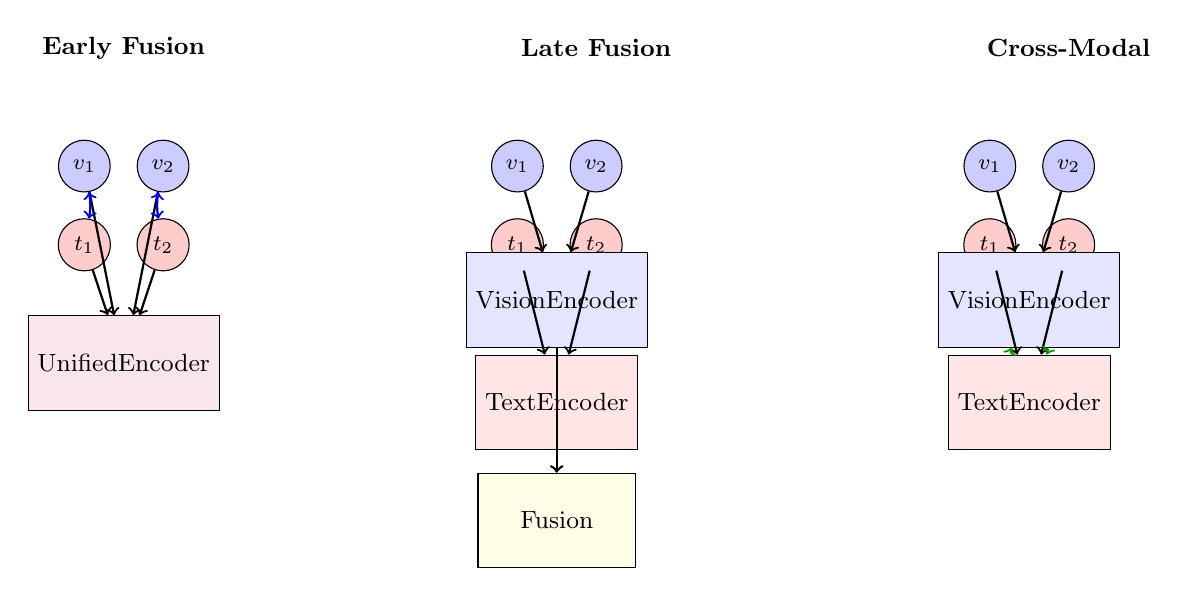
\begin{tikzpicture}[
  node/.style={circle, draw, minimum size=0.6cm, font=\footnotesize},
  encoder/.style={rectangle, draw, minimum width=2cm, minimum height=1.2cm, font=\small},
  arrow/.style={->, thick},
  bidir/.style={<->, thick, blue},
  cross/.style={->, thick, green!60!black, dashed}
]

% Early Fusion
\node[font=\small\bfseries] at (0,4) {Early Fusion};
\node[node, fill=blue!20] (v1) at (-0.5,2.5) {$v_1$};
\node[node, fill=blue!20] (v2) at (0.5,2.5) {$v_2$};
\node[node, fill=red!20] (t1) at (-0.5,1.5) {$t_1$};
\node[node, fill=red!20] (t2) at (0.5,1.5) {$t_2$};

\node[encoder, fill=purple!10] (enc1) at (0,0) {Unified \\ Encoder};
\draw[arrow] (v1) -- (enc1);
\draw[arrow] (v2) -- (enc1);
\draw[arrow] (t1) -- (enc1);
\draw[arrow] (t2) -- (enc1);

\draw[bidir] (v1) to[bend left=10] (t1);
\draw[bidir] (v2) to[bend right=10] (t2);


% Late Fusion
\node[font=\small\bfseries] at (6,4) {Late Fusion};
\node[node, fill=blue!20] (v3) at (5,2.5) {$v_1$};
\node[node, fill=blue!20] (v4) at (6,2.5) {$v_2$};
\node[node, fill=red!20] (t3) at (5,1.5) {$t_1$};
\node[node, fill=red!20] (t4) at (6,1.5) {$t_2$};

\node[encoder, fill=blue!10] (venc) at (5.5,0.8) {Vision \\ Encoder};
\node[encoder, fill=red!10] (tenc) at (5.5,-0.5) {Text \\ Encoder};

\draw[arrow] (v3) -- (venc);
\draw[arrow] (v4) -- (venc);
\draw[arrow] (t3) -- (tenc);
\draw[arrow] (t4) -- (tenc);

\node[encoder, fill=yellow!10] (fuse) at (5.5,-2) {Fusion};
\draw[arrow] (venc) -- (fuse);
\draw[arrow] (tenc) -- (fuse);


% Cross-Modal Attention
\node[font=\small\bfseries] at (12,4) {Cross-Modal};
\node[node, fill=blue!20] (v5) at (11,2.5) {$v_1$};
\node[node, fill=blue!20] (v6) at (12,2.5) {$v_2$};
\node[node, fill=red!20] (t5) at (11,1.5) {$t_1$};
\node[node, fill=red!20] (t6) at (12,1.5) {$t_2$};

\node[encoder, fill=blue!10] (venc2) at (11.5,0.8) {Vision \\ Encoder};
\node[encoder, fill=red!10] (tenc2) at (11.5,-0.5) {Text \\ Encoder};

\draw[arrow] (v5) -- (venc2);
\draw[arrow] (v6) -- (venc2);
\draw[arrow] (t5) -- (tenc2);
\draw[arrow] (t6) -- (tenc2);

\draw[cross] (venc2) to[bend left=20] (tenc2);
\draw[cross] (tenc2) to[bend left=20] (venc2);


\end{tikzpicture}
\caption{Three multimodal fusion strategies. \textbf{Early fusion} (left): concatenates modalities and processes with unified encoder, enabling rich interactions but with quadratic cost $O((N+M)^2)$. \textbf{Late fusion} (center): separate encoders with fusion only at output, efficient $O(N^2 + M^2)$ but limited cross-modal interaction. \textbf{Cross-modal attention} (right): separate encoders with explicit cross-attention, balancing efficiency $O(N^2 + M^2 + NM)$ with rich interactions.}
\label{fig:multimodal_fusion_strategies}
\end{figure}

\textbf{Early fusion} combines modalities at the input level, concatenating or interleaving embeddings from different sources before processing them through a single unified encoder. For example, an image might be encoded into a sequence of patch embeddings $\vv_1, \ldots, \vv_N \in \R^d$, while text is tokenized into embeddings $\vt_1, \ldots, \vt_M \in \R^d$. These are concatenated into a single sequence $[\vv_1, \ldots, \vv_N, \vt_1, \ldots, \vt_M]$ and processed by a standard transformer encoder. The advantage of this approach is its simplicity and the fact that cross-modal interactions can occur at every layer through self-attention. However, early fusion has significant computational drawbacks: the attention complexity is $O((N+M)^2 d)$, meaning that adding image patches dramatically increases the cost. For a ViT-Base image with 196 patches and text with 128 tokens, the combined sequence length of 324 tokens results in attention matrices of size $324 \times 324$, consuming substantial memory and compute compared to processing each modality separately.

\textbf{Late fusion} takes the opposite approach, using separate encoders for each modality and combining their outputs only at the final decision stage. An image encoder produces a single embedding $\vv \in \R^d$, a text encoder produces $\vt \in \R^d$, and these are combined through simple operations like concatenation, averaging, or element-wise multiplication before a final classification layer. This approach is computationally efficient since each encoder processes only its own modality with complexity $O(N^2 d)$ for images and $O(M^2 d)$ for text, which can be computed in parallel. The total complexity is $O(N^2 d + M^2 d)$ rather than $O((N+M)^2 d)$. However, late fusion severely limits cross-modal interactions—the encoders cannot attend to information from other modalities, and the combination happens only at the very end. This makes it difficult to learn fine-grained alignments, such as which image regions correspond to which words in a caption.

\textbf{Cross-modal attention} provides a middle ground, using separate encoders but introducing explicit attention mechanisms that allow one modality to query information from another. In this architecture, an image encoder produces a sequence of patch embeddings $\mV = [\vv_1, \ldots, \vv_N] \in \R^{N \times d}$, and a text encoder produces token embeddings $\mT = [\vt_1, \ldots, \vt_M] \in \R^{M \times d}$. Additional cross-attention layers are then inserted where text tokens attend to image patches (queries from text, keys and values from image) and vice versa. The computational cost is $O(N^2 d + M^2 d + NMd)$ for the self-attention in each modality plus the cross-attention between them. The cross-attention term $NMd$ is linear in both sequence lengths, making it much more efficient than early fusion's quadratic term. For our example with 196 image patches and 128 text tokens, cross-attention requires $196 \times 128 = 25{,}088$ attention computations per head, compared to $324^2 = 104{,}976$ for early fusion—a 4× reduction. This approach is used in models like BLIP and Flamingo, where it enables rich cross-modal interactions while maintaining computational tractability.

\subsection{Alignment Objectives}

\textbf{Contrastive Learning:}
\begin{equation}
\mathcal{L}_{\text{contrastive}} = -\log \frac{\exp(\text{sim}(v_i, t_i)/\tau)}{\sum_j \exp(\text{sim}(v_i, t_j)/\tau)}
\end{equation}
where $v_i$ = image embedding, $t_i$ = text embedding, $\tau$ = temperature

\textbf{Matching Loss:}
\begin{equation}
\mathcal{L}_{\text{match}} = -\mathbb{E}[\log P(\text{match}|v, t)]
\end{equation}

\textbf{Reconstruction:}
\begin{equation}
\mathcal{L}_{\text{recon}} = \|f_{\text{dec}}(v) - t\|^2
\end{equation}

\section{CLIP: Contrastive Language-Image Pre-training}
\label{sec:clip}

\subsection{CLIP Architecture}

CLIP (Contrastive Language-Image Pre-training) represents a breakthrough in vision-language learning by training image and text encoders jointly using a contrastive objective on 400 million image-text pairs collected from the internet. Unlike traditional supervised learning that requires manually labeled categories, CLIP learns to align images with their natural language descriptions, enabling zero-shot transfer to downstream tasks without any task-specific training data.

\begin{definition}[CLIP Model]
\label{def:clip}
The CLIP architecture consists of three main components that work together to create a shared embedding space for images and text. The \textbf{image encoder} can be either a Vision Transformer (ViT) or a ResNet, which processes an input image and produces a fixed-dimensional embedding $\vv \in \R^{d}$. For the largest CLIP model (ViT-L/14), the image encoder is a ViT with patch size 14, hidden dimension 1024, 24 layers, and 16 attention heads, totaling approximately 304 million parameters. The \textbf{text encoder} is a transformer decoder (similar to GPT) with a context length of 77 tokens, hidden dimension 768, 12 layers, and 12 attention heads, containing roughly 63 million parameters. Both encoders are followed by learned linear \textbf{projection layers} that map their outputs to a shared embedding space of dimension $d = 512$, where cosine similarity can be computed directly.

The training procedure processes batches of $(image, text)$ pairs simultaneously. For each batch of size $N$, all $N$ images are encoded to produce embeddings $\vv_1, \ldots, \vv_N \in \R^{512}$, and all $N$ text descriptions are encoded to produce $\vt_1, \ldots, \vt_N \in \R^{512}$. The model then computes an $N \times N$ similarity matrix where entry $(i,j)$ represents the cosine similarity between image $i$ and text $j$. The contrastive loss maximizes the similarity along the diagonal (correct image-text pairs) while minimizing off-diagonal similarities (incorrect pairings). This symmetric loss is computed in both directions—predicting text from image and image from text—and averaged.
\end{definition}

The parameter count for CLIP varies significantly across model scales. CLIP ResNet-50 contains approximately 102 million parameters (38M for ResNet-50 image encoder, 63M for text encoder, 1M for projections), while CLIP ViT-L/14 totals around 428 million parameters (304M for ViT-L image encoder, 123M for a larger text encoder with 768 dimensions and 12 layers, 1M for projections). The largest variant, ViT-L/14@336px, processes higher-resolution images (336×336 instead of 224×224) with the same architecture, increasing computational cost but improving performance on fine-grained tasks.

\begin{example}[CLIP Training]
\label{ex:clip_training}
Consider a training batch with size $N = 4$ and embedding dimension $d = 512$. The image encoder processes four images to produce embeddings arranged as rows in matrix $\mV = [\vv_1, \vv_2, \vv_3, \vv_4]\transpose \in \R^{4 \times 512}$, while the text encoder processes their corresponding captions to produce $\mT = [\vt_1, \vt_2, \vt_3, \vt_4]\transpose \in \R^{4 \times 512}$.

The similarity matrix is computed as $\mS = \mV \mT\transpose \in \R^{4 \times 4}$, where each entry $S_{ij}$ represents the dot product between image embedding $i$ and text embedding $j$. To make this scale-invariant, CLIP uses cosine similarity: $S_{ij} = \frac{\vv_i \cdot \vt_j}{\|\vv_i\| \|\vt_j\|}$, which normalizes each embedding to unit length before computing the dot product. This ensures that the similarity is determined by the angle between embeddings rather than their magnitudes.

The contrastive loss for the image-to-text direction is computed as:
\begin{equation}
\mathcal{L}_i^{\text{img}\to\text{txt}} = -\log \frac{\exp(S_{ii}/\tau)}{\sum_{j=1}^{N} \exp(S_{ij}/\tau)}
\end{equation}
where $\tau$ is a learned temperature parameter, initialized to $0.07$ and trained jointly with the model. The temperature controls the sharpness of the distribution: smaller values make the model more confident (sharper peaks), while larger values produce softer distributions. The symmetric text-to-image loss $\mathcal{L}_i^{\text{txt}\to\text{img}}$ is computed analogously by treating text as queries and images as candidates. The total loss averages both directions:
\begin{equation}
\mathcal{L} = \frac{1}{2N} \sum_{i=1}^{N} (\mathcal{L}_i^{\text{img}\to\text{txt}} + \mathcal{L}_i^{\text{txt}\to\text{img}})
\end{equation}

In practice, CLIP uses very large batch sizes to provide more negative examples for contrastive learning. The original CLIP was trained with batch size 32,768, requiring distributed training across multiple GPUs. With such large batches, each positive pair has 32,767 negative examples, providing a strong learning signal. However, this creates substantial memory requirements: storing the $32{,}768 \times 512$ embedding matrices for images and text requires $32{,}768 \times 512 \times 4 = 67$ MB per modality in FP32, and the $32{,}768 \times 32{,}768$ similarity matrix requires $4.3$ GB. To make this tractable, CLIP uses gradient checkpointing and distributes the batch across many GPUs, computing the similarity matrix in chunks.
\end{example}

\subsection{Computational Analysis of CLIP Training}

Training CLIP at scale requires careful consideration of computational and memory costs across both the image and text encoding paths. For the ViT-L/14 image encoder processing 224×224 images, each image is divided into $16 \times 16 = 256$ patches of size $14 \times 14$. These patches are linearly projected to dimension 1024 and processed through 24 transformer layers. The computational cost per image is approximately $2 \times 24 \times 256^2 \times 1024 = 3.2$ GFLOPS for the attention operations (using the $2Ld^2n^2$ formula from Chapter 12) plus $2 \times 24 \times 256 \times 4 \times 1024^2 = 51.5$ GFLOPS for the feed-forward networks, totaling roughly 55 GFLOPS per image.

The text encoder processes sequences of up to 77 tokens through 12 transformer layers with dimension 768. The computational cost per text is approximately $2 \times 12 \times 77^2 \times 768 = 1.1$ GFLOPS for attention plus $2 \times 12 \times 77 \times 4 \times 768^2 = 4.4$ GFLOPS for feed-forward networks, totaling about 5.5 GFLOPS per text. This asymmetry—images requiring 10× more compute than text—means that image encoding dominates the computational budget during training.

For a batch of 32,768 examples, the total forward pass requires approximately $32{,}768 \times (55 + 5.5) = 1{,}982{,}464$ GFLOPS or roughly 2 PFLOPS. On an NVIDIA A100 GPU with 312 TFLOPS of FP16 compute, this would take approximately 6.4 seconds per batch for the forward pass alone, not including backward propagation (which typically costs 2× the forward pass) or the contrastive loss computation. The full training of CLIP on 400 million image-text pairs with batch size 32,768 requires approximately $400{,}000{,}000 / 32{,}768 = 12{,}207$ batches. At roughly 20 seconds per batch (forward + backward + optimizer step), this amounts to 68 hours of continuous training on a single A100. In practice, OpenAI trained CLIP on 256 V100 GPUs for approximately 12 days, suggesting a total training cost of around 73,728 GPU-hours.

Memory requirements are equally demanding. Each image in the batch requires storing activations for 24 layers with 256 tokens and dimension 1024, totaling approximately $24 \times 256 \times 1024 \times 2 = 12.6$ MB per image in FP16 (the factor of 2 accounts for storing both pre- and post-activation values for backpropagation). For batch size 32,768, this amounts to 413 GB just for image activations. Text activations are smaller at approximately $12 \times 77 \times 768 \times 2 = 1.4$ MB per text, or 46 GB for the full batch. The similarity matrix requires $32{,}768 \times 32{,}768 \times 2 = 2.1$ GB in FP16. Combined with model parameters (428M parameters × 2 bytes = 856 MB) and optimizer states (typically 2× parameters for Adam), the total memory footprint exceeds 500 GB, necessitating distribution across many GPUs using techniques like ZeRO (Chapter 22) to partition optimizer states and activations.

\subsection{Zero-Shot Classification with CLIP}

One of CLIP's most remarkable capabilities is zero-shot classification: the ability to classify images into categories the model has never been explicitly trained on. This works by leveraging the natural language understanding of the text encoder to create classifiers on the fly from text descriptions. The procedure begins by creating text prompts for each class in the target classification task. For example, for a 10-class animal classification task, we might create prompts like "a photo of a dog", "a photo of a cat", "a photo of a bird", and so on. These prompts are encoded by the text encoder to produce class embeddings $\vt_1, \ldots, \vt_C \in \R^{512}$ where $C$ is the number of classes.

To classify a new image, we encode it with the image encoder to produce $\vv \in \R^{512}$, then compute the cosine similarity between the image embedding and each class embedding: $s_i = \frac{\vv \cdot \vt_i}{\|\vv\| \|\vt_i\|}$. The predicted class is simply $\arg\max_i s_i$, the class whose text description has the highest similarity to the image. This approach requires no training on the target dataset—the model uses only its pre-trained knowledge of how images and text relate.

The performance of this zero-shot approach is surprisingly strong. CLIP ViT-L/14 achieves 76.2\% top-1 accuracy on ImageNet without ever seeing a single ImageNet training example, matching the performance of a ResNet-50 trained directly on ImageNet's 1.28 million labeled images. This demonstrates that CLIP has learned visual concepts that generalize far beyond its training distribution. Moreover, CLIP shows remarkable robustness to distribution shift: when evaluated on ImageNet variants with different image styles (sketches, cartoons, adversarial examples), CLIP's performance degrades much less than supervised models, suggesting it has learned more robust visual representations.

The prompt engineering aspect of zero-shot classification is crucial for performance. Simple prompts like "dog" perform worse than more descriptive prompts like "a photo of a dog". OpenAI found that using prompt ensembles—averaging predictions across multiple prompt templates like "a photo of a \{class\}", "a picture of a \{class\}", "an image of a \{class\}"—improves accuracy by 1-2\% by reducing sensitivity to prompt phrasing. For fine-grained classification tasks, more specific prompts help: "a photo of a \{species\}, a type of bird" outperforms "a photo of a \{species\}" for bird species classification.

\subsection{CLIP Variants and Training Requirements}

Following CLIP's success, several variants have been developed with different scales and training procedures. \textbf{OpenCLIP} is an open-source reproduction that has trained models ranging from small (ResNet-50 with 102M parameters) to very large (ViT-G/14 with 1.8B parameters) on datasets including LAION-400M and LAION-2B. The largest OpenCLIP models require training on clusters of 128-512 A100 GPUs for several weeks, with estimated costs exceeding \$100,000 for the full training run. The training uses mixed precision (FP16) to reduce memory consumption and enable larger batch sizes, typically 32,768 to 65,536 examples distributed across all GPUs.

\textbf{ALIGN}, developed by Google, scales up the training data to 1.8 billion noisy image-text pairs collected from the web without extensive filtering. This demonstrates that contrastive learning is robust to noise in the training data—the model learns to ignore mismatched pairs through the contrastive objective. ALIGN uses an EfficientNet-L2 image encoder (480M parameters) and a BERT-Large text encoder (340M parameters), totaling approximately 820M parameters. Training ALIGN required a cluster of 1024 Cloud TPU v3 cores for approximately 6 days, representing roughly 150,000 TPU-hours.

\textbf{Florence}, Microsoft's unified vision foundation model, extends the CLIP approach to 900 million image-text pairs with a focus on creating a single model that can be adapted to diverse vision tasks. Florence uses a CoSwin transformer as the image encoder (637M parameters) and achieves state-of-the-art results on zero-shot classification, retrieval, and object detection after fine-tuning. The training infrastructure required 512 NVIDIA A100 GPUs for approximately 10 days, with an estimated cost of over \$200,000 in cloud compute.

The hardware requirements for training CLIP-scale models are substantial. A minimum viable setup might use 8-16 A100 GPUs (80GB each) to train a CLIP ResNet-50 model on a smaller dataset like Conceptual Captions (3M pairs) with batch size 2048-4096, requiring approximately 1-2 weeks. Scaling to the full CLIP ViT-L/14 with 400M training pairs and batch size 32,768 necessitates at least 64-128 A100 GPUs with high-bandwidth interconnects (NVLink or InfiniBand) to efficiently synchronize gradients across the distributed batch. The total training cost for reproducing CLIP ViT-L/14 is estimated at \$50,000-\$100,000 in cloud GPU costs, depending on the provider and optimization techniques employed.

\section{DALL-E and Stable Diffusion}
\label{sec:dalle}

\subsection{DALL-E: Text-to-Image Generation}

\begin{definition}[DALL-E Architecture]
\label{def:dalle}
\textbf{DALL-E 1 (2021):}
\begin{itemize}
    \item Encoder: Compress images to discrete tokens (VQ-VAE)
    \item Transformer: Autoregressive model over text + image tokens
    \item Training: Next token prediction
\end{itemize}

\textbf{Sequence:}
\begin{equation}
[\text{BOS}, \text{text tokens}, \text{image tokens}, \text{EOS}]
\end{equation}

Generate image by: (1) Encode text, (2) Sample image tokens autoregressively
\end{definition}

\textbf{DALL-E 2 (2022):}
\begin{itemize}
    \item Use CLIP embeddings
    \item Prior: Text embedding $\to$ Image embedding
    \item Decoder: Image embedding $\to$ Image (diffusion model)
    \item Much higher quality than DALL-E 1
\end{itemize}

\subsection{Stable Diffusion}

\textbf{Latent Diffusion Model:}
\begin{enumerate}
    \item Encode image to latent space (VAE)
    \item Add noise iteratively (forward diffusion)
    \item Learn to denoise (reverse diffusion)
    \item Condition on text via cross-attention
\end{enumerate}

\textbf{Text conditioning:}
\begin{itemize}
    \item Text encoder: CLIP or T5
    \item Cross-attention: Latent queries attend to text keys/values
    \item Enables text-guided image generation
\end{itemize}

\begin{example}[Stable Diffusion Architecture]
\label{ex:stable_diffusion}
\textbf{Components:}

\textbf{1. Text Encoder:} CLIP text encoder
\begin{equation}
\text{prompt} \to \vt \in \R^{77 \times 768}
\end{equation}

\textbf{2. VAE Encoder:} Image $\to$ latent
\begin{equation}
\mI \in \R^{512 \times 512 \times 3} \to \vz \in \R^{64 \times 64 \times 4}
\end{equation}

\textbf{3. U-Net Denoiser:} Diffusion model with cross-attention
\begin{itemize}
    \item Input: Noisy latent $\vz_t$
    \item Condition: Text embedding $\vt$
    \item Output: Predicted noise $\epsilon_\theta(\vz_t, t, \vt)$
\end{itemize}

\textbf{4. VAE Decoder:} Latent $\to$ image
\begin{equation}
\vz \in \R^{64 \times 64 \times 4} \to \mI \in \R^{512 \times 512 \times 3}
\end{equation}

\textbf{Parameters:} $\approx 860$M total
\end{example}

\section{Vision-Language Understanding}
\label{sec:vision_language_understanding}

\subsection{BLIP: Bootstrapped Language-Image Pre-training}

\textbf{Architecture:}
\begin{itemize}
    \item Image encoder (ViT)
    \item Text encoder (BERT)
    \item Multimodal encoder (cross-attention between vision and text)
\end{itemize}

\textbf{Training objectives:}
\begin{enumerate}
    \item \textbf{ITC:} Image-Text Contrastive (like CLIP)
    \item \textbf{ITM:} Image-Text Matching (binary: match or not)
    \item \textbf{LM:} Language Modeling on text
\end{enumerate}

\textbf{Bootstrapping:} Generate synthetic captions, filter with model, retrain

\subsection{Flamingo: Few-Shot Learning}

Flamingo represents a significant architectural innovation in multimodal transformers by enabling models to process arbitrarily interleaved sequences of images and text, supporting few-shot learning through in-context examples. Unlike CLIP, which processes single image-text pairs, Flamingo can handle inputs like "Here is an image of a cat: \texttt{<image1>}. Here is an image of a dog: \texttt{<image2>}. What animal is in this image: \texttt{<image3>}?" This capability enables few-shot visual learning where the model learns new tasks from just a few examples provided in the prompt, without any parameter updates.

The Flamingo architecture consists of three main components, carefully designed to leverage pre-trained models while adding minimal trainable parameters. The \textbf{vision encoder} is a frozen CLIP ViT-L/14 model that processes each image independently to produce a sequence of patch embeddings. For a 224×224 image with patch size 14, this yields 256 patch tokens of dimension 1024. The vision encoder's 304M parameters remain frozen throughout training, preserving the strong visual representations learned during CLIP pre-training.

The \textbf{language model} is a frozen Chinchilla 70B model, a large autoregressive transformer trained on text-only data. Chinchilla uses 70 billion parameters across 80 layers with hidden dimension 8192 and 64 attention heads. Keeping this massive language model frozen is crucial for computational tractability—training 70B parameters would require prohibitive memory and compute. Instead, Flamingo inserts new trainable layers that allow the frozen language model to attend to visual information without modifying its core text processing capabilities.

The key innovation is the \textbf{Perceiver Resampler}, a learned module that compresses the variable-length sequence of image patch embeddings into a fixed number of visual tokens that can be efficiently processed by the language model. The Perceiver Resampler uses cross-attention where a fixed set of learned queries $\mQ \in \R^{64 \times 2048}$ (64 visual tokens, dimension 2048) attends to the image patch embeddings $\mK, \mV \in \R^{256 \times 1024}$ from the vision encoder. This produces a fixed-size representation regardless of input image resolution or the number of images in the sequence. The Perceiver Resampler contains approximately 1.4B parameters (6 layers of cross-attention and feed-forward networks with dimension 2048), making it the primary trainable component of Flamingo.

Between every few layers of the frozen language model, Flamingo inserts new \textbf{cross-attention layers} that allow text tokens to attend to the visual tokens produced by the Perceiver Resampler. Specifically, for Flamingo-80B (built on Chinchilla-70B), cross-attention layers are inserted after every 7th transformer layer, resulting in approximately 11 cross-attention insertions across the 80 layers. Each cross-attention layer adds roughly 134M parameters (for dimension 8192), totaling about 1.5B parameters for all insertions. Combined with the Perceiver Resampler, Flamingo adds approximately 2.9B trainable parameters to the 70B frozen base model, representing just 4\% additional parameters while enabling full multimodal capabilities.

The memory requirements for Flamingo are dominated by the frozen language model. Storing 70B parameters in FP16 requires 140 GB, which exceeds the memory of any single GPU. Flamingo uses model parallelism to partition the language model across multiple GPUs—for example, distributing across 8 A100 GPUs (80GB each) places roughly 8.75B parameters per GPU, consuming about 17.5 GB for parameters. Activations for a sequence of 2048 tokens (including both text and visual tokens) across 80 layers with dimension 8192 require approximately $2048 \times 80 \times 8192 \times 2 = 2.6$ GB per example in FP16. With batch size 8, activations consume 21 GB per GPU, leaving sufficient memory for gradients of the trainable parameters (2.9B parameters × 2 bytes × 2 for gradients = 11.6 GB) and optimizer states (23.2 GB for Adam).

Training Flamingo on a mixture of image-text pairs, interleaved image-text documents, and video-text pairs requires substantial computational resources. The training dataset consists of 2.3 billion image-text pairs (similar to CLIP), 43 million interleaved image-text web pages, and 27 million video clips. Training Flamingo-80B for 1 epoch through this data with batch size 256 distributed across 256 A100 GPUs takes approximately 15 days, representing roughly 92,000 GPU-hours. The estimated training cost exceeds \$300,000 in cloud compute. However, the key advantage is that only 2.9B parameters are trained while leveraging the capabilities of a 70B language model, making training far more efficient than training a 70B multimodal model from scratch.

For inference, Flamingo's few-shot learning capability means that users can provide 2-32 example image-text pairs in the prompt to demonstrate a new task, and the model adapts its predictions based on these examples without any fine-tuning. This in-context learning works because the cross-attention mechanism allows the model to attend to the example images when processing the query image. The computational cost of inference scales linearly with the number of examples in the context: each additional image adds 256 patch tokens (after vision encoding) compressed to 64 visual tokens (after Perceiver Resampler), increasing the sequence length and thus the attention cost. For a prompt with 4 example images and 1 query image (5 images total), the visual tokens contribute $5 \times 64 = 320$ tokens to the sequence, which combined with text tokens (typically 500-1000) results in sequences of 800-1300 tokens. On a single A100 GPU, Flamingo-80B can process approximately 2-3 such sequences per second, limited primarily by the memory bandwidth required to load the 70B parameter model.

\section{Computational Analysis of Multimodal Transformers}
\label{sec:multimodal_computational_analysis}

\subsection{Image Encoding Cost}

The computational cost of encoding images in multimodal transformers depends critically on the choice of vision encoder architecture and input resolution. For a Vision Transformer processing an image of resolution $H \times W$ with patch size $P$, the image is divided into $n = \frac{HW}{P^2}$ patches. Each patch is linearly projected to dimension $d$, and the resulting sequence of $n$ tokens is processed through $L$ transformer layers. The total computational cost is approximately $2Ld^2n^2$ FLOPs for attention operations plus $8Ld^2n$ FLOPs for feed-forward networks (using the standard 4× expansion ratio).

For concrete analysis, consider three common configurations. A ViT-Base model with 224×224 images, patch size 16, dimension 768, and 12 layers processes $n = 196$ patches. The attention cost is $2 \times 12 \times 768^2 \times 196^2 = 5.5$ GFLOPs, and the feed-forward cost is $8 \times 12 \times 768^2 \times 196 = 11.0$ GFLOPs, totaling 16.5 GFLOPs per image. A ViT-Large model with patch size 14, dimension 1024, and 24 layers processes $n = 256$ patches, requiring approximately $2 \times 24 \times 1024^2 \times 256^2 = 3.2$ TFLOPs for attention and $8 \times 24 \times 1024^2 \times 256 = 51.5$ GFLOPs for feed-forward, totaling 3.25 TFLOPs per image—nearly 200× more than ViT-Base. Increasing resolution to 336×336 (as in CLIP ViT-L/14@336px) increases the patch count to $n = 576$, quadrupling the attention cost to 14.4 TFLOPs and more than doubling the total cost to 14.5 TFLOPs per image.

The memory requirements for image encoding are dominated by storing activations for backpropagation during training. For ViT-Large processing 256 patches through 24 layers with dimension 1024, each layer stores attention outputs ($256 \times 1024$), feed-forward outputs ($256 \times 4096$ intermediate, $256 \times 1024$ output), and layer norm statistics. Accounting for all activations, each image requires approximately $24 \times 256 \times (1024 + 4096 + 1024) \times 2 = 75$ MB in FP16. For a batch of 256 images (typical for CLIP training when distributed across many GPUs), activations consume 19.2 GB per GPU, leaving limited memory for model parameters and optimizer states on a 40GB A100 GPU.

\subsection{Text Encoding Cost}

Text encoding is typically far less expensive than image encoding due to shorter sequence lengths. For a transformer processing text with sequence length $m$ tokens through $L$ layers with dimension $d$, the computational cost is $2Ld^2m^2$ for attention plus $8Ld^2m$ for feed-forward networks. The CLIP text encoder uses $m = 77$ tokens, $d = 768$, and $L = 12$ layers, resulting in attention cost $2 \times 12 \times 768^2 \times 77^2 = 1.1$ GFLOPs and feed-forward cost $8 \times 12 \times 768^2 \times 77 = 4.4$ GFLOPs, totaling 5.5 GFLOPs per text—approximately 10× less than encoding a single image with ViT-Large.

However, for large language models used in architectures like Flamingo, text encoding becomes more expensive. Chinchilla-70B uses 80 layers with dimension 8192, processing sequences of up to 2048 tokens. The attention cost is $2 \times 80 \times 8192^2 \times 2048^2 = 1.1 \times 10^{17}$ FLOPs or 110 PFLOPs per sequence, and the feed-forward cost is $8 \times 80 \times 8192^2 \times 2048 = 8.8$ TFLOPs, totaling approximately 110 TFLOPs per sequence. This is 34,000× more expensive than the CLIP text encoder and 34× more expensive than ViT-Large image encoding, demonstrating how large language models dominate the computational budget in models like Flamingo.

Memory for text activations scales with sequence length and model size. For Chinchilla-70B processing 2048 tokens through 80 layers with dimension 8192, storing activations requires approximately $80 \times 2048 \times (8192 + 32768 + 8192) \times 2 = 13$ GB per sequence in FP16 (accounting for attention outputs, feed-forward intermediate activations with 4× expansion, and final outputs). With batch size 8 distributed across 8 GPUs, each GPU stores activations for 1 sequence, consuming 13 GB of the 80 GB available on an A100.

\subsection{Cross-Modal Attention Cost}

Cross-modal attention, where one modality attends to another, introduces additional computational costs that scale with the product of sequence lengths from both modalities. For text tokens attending to image patches, the attention operation computes $\mQ \mK\transpose$ where $\mQ \in \R^{m \times d}$ (text queries) and $\mK \in \R^{n \times d}$ (image keys), producing an attention matrix of size $m \times n$. The computational cost is $2mnd$ FLOPs for the matrix multiplication, plus $2mnd$ for computing the weighted sum with values, totaling $4mnd$ FLOPs per cross-attention layer.

For a model like BLIP with $m = 128$ text tokens, $n = 196$ image patches, and $d = 768$, each cross-attention layer costs $4 \times 128 \times 196 \times 768 = 77$ MFLOPs. With 6 cross-attention layers in the multimodal encoder, the total cross-attention cost is 462 MFLOPs—negligible compared to the self-attention costs in the image and text encoders. However, the memory for storing the $m \times n$ attention matrices is $128 \times 196 \times 2 = 50$ KB per layer in FP16, or 300 KB for 6 layers, which is also minimal.

In Flamingo, the cross-attention cost is higher due to the large language model dimension. With $m = 2048$ text tokens, $n = 64$ visual tokens (after Perceiver Resampler compression), and $d = 8192$, each cross-attention layer costs $4 \times 2048 \times 64 \times 8192 = 4.3$ GFLOPs. With approximately 11 cross-attention layers inserted throughout the 80-layer language model, the total cross-attention cost is 47 GFLOPs per forward pass. While this is small compared to the 110 TFLOPs for the language model self-attention, it represents a non-trivial addition. The memory for attention matrices is $2048 \times 64 \times 2 = 262$ KB per layer, or 2.9 MB for all 11 layers—again minimal compared to activation memory.

\subsection{Total Memory Requirements}

The total memory footprint for training multimodal transformers includes model parameters, activations, gradients, and optimizer states. For CLIP ViT-L/14 with 428M parameters, the parameters require $428 \times 10^6 \times 2 = 856$ MB in FP16. Gradients require an additional 856 MB. The Adam optimizer maintains two states (momentum and variance) per parameter, requiring $428 \times 10^6 \times 4 = 1.7$ GB in FP32 (optimizer states are typically kept in higher precision for numerical stability). Activations for a batch of 256 images and 256 texts consume approximately $256 \times (75 + 1.4) = 19.6$ GB as calculated earlier. The total memory per GPU is approximately $0.9 + 0.9 + 1.7 + 19.6 = 23.1$ GB, fitting comfortably on a 40GB A100 GPU.

For Flamingo-80B, the memory requirements are far more demanding. The 70B frozen parameters require $70 \times 10^9 \times 2 = 140$ GB in FP16, necessitating distribution across at least 2 A100 GPUs (80GB each). The 2.9B trainable parameters require $2.9 \times 10^9 \times 2 = 5.8$ GB for parameters, 5.8 GB for gradients, and $2.9 \times 10^9 \times 4 = 11.6$ GB for optimizer states, totaling 23.2 GB. Activations for a sequence of 2048 tokens through 80 layers with dimension 8192 require approximately 13 GB per sequence as calculated earlier. For batch size 8 distributed across 8 GPUs (1 sequence per GPU), the total memory per GPU is approximately $140/8 + 23.2 + 13 = 53.7$ GB, fitting on an 80GB A100 but leaving limited headroom. In practice, Flamingo uses gradient checkpointing to reduce activation memory by recomputing activations during backpropagation, trading compute for memory and enabling larger batch sizes or longer sequences.

\section{Training Challenges for Multimodal Transformers}
\label{sec:multimodal_training_challenges}

\subsection{Batch Size Requirements for Contrastive Learning}

Contrastive learning methods like CLIP require very large batch sizes to provide sufficient negative examples for effective learning. The contrastive loss compares each positive image-text pair against all other pairs in the batch, treating them as negatives. With batch size $N$, each example has $N-1$ negative examples, and the quality of the learned representations improves significantly as $N$ increases. Empirically, CLIP's performance scales log-linearly with batch size: increasing from 256 to 32,768 improves ImageNet zero-shot accuracy from approximately 58\% to 76\%, a gain of 18 percentage points.

However, large batch sizes create severe memory constraints. For batch size 32,768 with CLIP ViT-L/14, storing the image embeddings requires $32{,}768 \times 512 \times 4 = 67$ MB in FP32 (embeddings are kept in FP32 for numerical stability in the contrastive loss computation). Text embeddings require another 67 MB. The $32{,}768 \times 32{,}768$ similarity matrix requires $32{,}768^2 \times 4 = 4.3$ GB in FP32. During backpropagation, gradients of the loss with respect to the similarity matrix also require 4.3 GB. The total memory for just the contrastive loss computation is approximately 8.7 GB, not including model parameters, activations, or optimizer states.

To make such large batches tractable, CLIP uses distributed training across many GPUs with careful memory management. Each GPU processes a local batch of size $N_{\text{local}} = N / G$ where $G$ is the number of GPUs. For $N = 32{,}768$ distributed across 256 GPUs, each GPU processes 128 examples. The key insight is that the similarity matrix can be computed in a distributed fashion: each GPU computes similarities between its local images and all texts (gathered from all GPUs via all-gather communication), producing a $128 \times 32{,}768$ matrix that requires only $128 \times 32{,}768 \times 4 = 16.8$ MB per GPU. The full $32{,}768 \times 32{,}768$ matrix is never materialized on any single GPU, reducing memory requirements by a factor of $G$.

The communication cost for distributed contrastive learning is substantial. Each GPU must perform an all-gather operation to collect embeddings from all other GPUs, communicating $32{,}768 \times 512 \times 4 = 67$ MB for images and 67 MB for text, totaling 134 MB per GPU per training step. With high-bandwidth interconnects like NVLink (300 GB/s) or InfiniBand (200 Gb/s = 25 GB/s), this communication takes approximately 5-10 milliseconds. For comparison, the forward and backward pass through the model takes approximately 50-100 milliseconds per step, so communication overhead is 5-10\% of the total training time—significant but not prohibitive.

\subsection{Memory Optimization Techniques}

Beyond distributed training, several memory optimization techniques are essential for training large multimodal models. \textbf{Gradient checkpointing} trades computation for memory by not storing all activations during the forward pass. Instead, only a subset of activations (typically at layer boundaries) are stored, and intermediate activations are recomputed during backpropagation when needed. For CLIP ViT-L/14, gradient checkpointing reduces activation memory from approximately 75 MB per image to 25 MB per image (a 3× reduction) at the cost of increasing training time by approximately 20\% due to recomputation. This enables increasing batch size from 128 to 384 per GPU, which more than compensates for the slowdown by improving convergence.

\textbf{Mixed precision training} uses FP16 for most computations while maintaining FP32 master weights and loss scaling to prevent gradient underflow. For multimodal transformers, this reduces activation memory by 50\% and accelerates matrix multiplications on modern GPUs with Tensor Cores. CLIP training with mixed precision reduces memory from 23.1 GB to approximately 14.5 GB per GPU, enabling batch sizes of 256 per GPU instead of 128. The training speedup is approximately 1.8× on A100 GPUs, reducing total training time from 12 days to 7 days on the same hardware.

\textbf{ZeRO (Zero Redundancy Optimizer)} partitions optimizer states, gradients, and optionally parameters across GPUs to reduce per-GPU memory consumption. For Flamingo-80B with 2.9B trainable parameters, the optimizer states alone require 11.6 GB per GPU without ZeRO. With ZeRO Stage 2 (partitioning optimizer states and gradients), this is reduced to $11.6 / G$ GB per GPU where $G$ is the number of GPUs. With 8 GPUs, optimizer memory drops from 11.6 GB to 1.45 GB per GPU, freeing memory for larger batch sizes or longer sequences. ZeRO Stage 3 additionally partitions parameters, reducing the 5.8 GB parameter memory to 0.73 GB per GPU, though this increases communication overhead as parameters must be gathered during forward and backward passes.

\subsection{Distributed Training Infrastructure}

Training multimodal transformers at scale requires sophisticated distributed training infrastructure with high-bandwidth interconnects and efficient parallelism strategies. For CLIP-scale models (400M parameters, 400M training examples), a typical setup uses 64-256 A100 GPUs connected via NVLink within nodes and InfiniBand between nodes. Each node contains 8 GPUs with NVLink providing 600 GB/s bidirectional bandwidth between GPUs in the same node, while InfiniBand provides 200 Gb/s (25 GB/s) between nodes. This hierarchical network topology means that communication within a node is 24× faster than between nodes, making it crucial to minimize cross-node communication.

The parallelism strategy combines data parallelism (different GPUs process different data) with model parallelism (different GPUs hold different parts of the model). For CLIP, pure data parallelism is typically sufficient since the model fits on a single GPU. Each GPU holds a full copy of the 428M parameter model (856 MB in FP16) and processes a local batch of images and texts. Gradients are synchronized across all GPUs using all-reduce operations after each backward pass, communicating $428 \times 10^6 \times 2 = 856$ MB per GPU. With 256 GPUs and ring all-reduce, this takes approximately $856 \text{ MB} \times 2 \times (256-1) / 256 / 25 \text{ GB/s} = 68$ ms, adding roughly 10-15\% overhead to the training step time.

For Flamingo-80B, model parallelism is essential since the 70B parameter language model cannot fit on a single GPU. The model is partitioned across 8 GPUs using tensor parallelism, where each linear layer's weight matrix is split across GPUs. For a linear layer with weight $\mW \in \R^{8192 \times 8192}$, each GPU holds $\mW_i \in \R^{8192 \times 1024}$ (1/8th of the columns). During the forward pass, each GPU computes a partial output, then an all-reduce operation sums the results. This requires communicating $8192 \times 2 = 16$ KB per linear layer, which is minimal. However, with hundreds of linear layers across 80 transformer layers, the cumulative communication overhead is approximately 5-10\% of training time.

\subsection{Training Time and Cost Estimates}

The total training time for multimodal transformers depends on the number of training examples, batch size, model size, and hardware configuration. For CLIP ViT-L/14 trained on 400M image-text pairs with batch size 32,768, the number of training steps is $400{,}000{,}000 / 32{,}768 = 12{,}207$ steps. Each step requires a forward pass (approximately 2 PFLOPs as calculated earlier), backward pass (approximately 4 PFLOPs, twice the forward pass), and optimizer step (negligible compute). The total compute is approximately $12{,}207 \times 6 \text{ PFLOPs} = 73{,}242$ PFLOPs.

On an NVIDIA A100 GPU with 312 TFLOPS of FP16 compute and approximately 50\% utilization (accounting for memory bandwidth limitations and non-compute operations), the effective throughput is 156 TFLOPS. Training on a single A100 would take $73{,}242 \text{ PFLOPs} / 156 \text{ TFLOPS} = 469{,}500$ seconds or approximately 130 hours. However, this ignores memory constraints—a single A100 cannot hold the activations for batch size 32,768. With 256 A100 GPUs, the training time is approximately $130 / 256 = 0.5$ hours, but this assumes perfect scaling, which is unrealistic due to communication overhead. In practice, with 10-15\% communication overhead, the training time is approximately 0.6 hours per epoch. For multiple epochs (CLIP was trained for approximately 32 epochs), the total training time is approximately 19 hours on 256 A100 GPUs, though the actual training took several days due to additional factors like data loading, checkpointing, and debugging.

The cost of training CLIP at cloud pricing can be estimated from GPU-hours. Training for 19 hours on 256 A100 GPUs requires $19 \times 256 = 4{,}864$ GPU-hours. At typical cloud pricing of \$2.50-\$4.00 per A100 GPU-hour, the total cost is approximately \$12,000-\$19,000 for a single training run. However, the actual development cost is much higher due to hyperparameter tuning, ablation studies, and failed experiments. OpenAI likely spent 10-20× this amount in total compute to develop CLIP, suggesting a total cost of \$120,000-\$380,000.

For Flamingo-80B, the training cost is substantially higher due to the 70B parameter language model. Training on 2.3B image-text pairs plus interleaved documents with batch size 256 distributed across 256 A100 GPUs for approximately 15 days requires $15 \times 24 \times 256 = 92{,}160$ GPU-hours. At \$3.00 per A100 GPU-hour, the total cost is approximately \$276,000 for a single training run. Including development costs, the total investment in training Flamingo likely exceeded \$1 million in compute costs alone, not including researcher time, data collection, and infrastructure development.

\section{Audio Transformers}
\label{sec:audio_transformers}

\subsection{Whisper: Speech Recognition}

\begin{definition}[Whisper Architecture]
\label{def:whisper}
Encoder-decoder transformer for speech:

\textbf{Input:} Audio waveform $\to$ Log-mel spectrogram

\textbf{Encoder:}
\begin{itemize}
    \item Input: Spectrogram (80 mel bins)
    \item Convolution layers (downsample)
    \item Transformer encoder layers
\end{itemize}

\textbf{Decoder:}
\begin{itemize}
    \item Autoregressive text generation
    \item Special tokens for language, task, timestamps
\end{itemize}
\end{definition}

\textbf{Training data:} 680,000 hours of multilingual audio

\textbf{Tasks supported:}
\begin{itemize}
    \item Speech recognition (transcription)
    \item Translation (to English)
    \item Language identification
    \item Voice activity detection
    \item Timestamp prediction
\end{itemize}

\begin{example}[Whisper Input Format]
\label{ex:whisper_format}
\textbf{Special tokens:}
\begin{verbatim}
<|startoftranscript|><|en|><|transcribe|><|notimestamps|>
\end{verbatim}

\textbf{Spectrogram:}
\begin{itemize}
    \item 80 mel bins
    \item 3000 frames (30 seconds audio at 100 Hz)
    \item Input: $3000 \times 80$
\end{itemize}

\textbf{Encoder:}
\begin{itemize}
    \item Conv layers: $3000 \times 80 \to 1500 \times 768$
    \item Transformer: Process 1500 tokens
\end{itemize}

\textbf{Decoder:} Generate text tokens autoregressively
\end{example}

\subsection{Audio-Text Pre-training}

\textbf{Contrastive learning:} Like CLIP but audio-text

\textbf{AudioCLIP:} Tri-modal (image, text, audio)

\textbf{Applications:}
\begin{itemize}
    \item Zero-shot audio classification
    \item Audio captioning
    \item Text-to-audio generation
\end{itemize}

\section{Unified Multimodal Models}
\label{sec:unified_multimodal}

\subsection{Perceiver and Perceiver IO}

\textbf{Key idea:} Map arbitrary modalities to latent space via cross-attention

\begin{definition}[Perceiver]
\label{def:perceiver}
\textbf{Components:}

\textbf{1. Latent array:} Fixed set of learned queries $\mZ \in \R^{M \times d}$

\textbf{2. Cross-attention:} Latents attend to inputs
\begin{equation}
\mZ_1 = \text{CrossAttn}(\mQ=\mZ, \mK=\mX, \mV=\mX)
\end{equation}

\textbf{3. Transformer:} Process latents
\begin{equation}
\mZ_L = \text{Transformer}(\mZ_1)
\end{equation}

\textbf{4. Output:} Decode latents to task outputs
\end{definition}

\textbf{Benefits:}
\begin{itemize}
    \item Handles arbitrary input sizes
    \item Computation independent of input size (fixed latents)
    \item Unified architecture for images, video, audio, text
\end{itemize}

\subsection{GPT-4V and LLaVA}

\textbf{GPT-4V (Vision):} GPT-4 with vision capabilities
\begin{itemize}
    \item Interleaved image and text inputs
    \item Strong vision-language understanding
    \item Details not fully disclosed
\end{itemize}

\textbf{LLaVA (Open-source):}
\begin{itemize}
    \item CLIP vision encoder
    \item LLaMA language model
    \item Linear projection to align embeddings
    \item Instruction tuning on visual conversations
\end{itemize}

\section{Exercises}

\begin{exercise}
Implement CLIP contrastive loss for batch size 8:
\begin{enumerate}
    \item Generate random image embeddings $(8, 512)$
    \item Generate random text embeddings $(8, 512)$
    \item Compute $8 \times 8$ similarity matrix
    \item Calculate contrastive loss with $\tau = 0.07$
\end{enumerate}
\end{exercise}

\begin{exercise}
Use CLIP for zero-shot classification on CIFAR-10:
\begin{enumerate}
    \item Load pre-trained CLIP model
    \item Create text prompts for 10 classes
    \item Encode images and prompts
    \item Compute accuracy
    \item Compare to supervised baseline
\end{enumerate}
\end{exercise}

\begin{exercise}
Analyze Whisper architecture:
\begin{enumerate}
    \item Calculate parameters for encoder (24 layers, $d=1024$)
    \item Calculate parameters for decoder (24 layers)
    \item Estimate memory for 30-second audio
    \item Compare to text-only GPT-2
\end{enumerate}
\end{exercise}

\begin{exercise}
Design multimodal fusion strategy for video understanding (visual + audio + captions):
\begin{enumerate}
    \item Propose architecture
    \item Define fusion mechanism
    \item Specify training objective
    \item Estimate parameter count
\end{enumerate}
\end{exercise}



\section{Solutions}

\begin{solution}
\textbf{Exercise 1: CLIP Contrastive Loss Implementation}

\begin{lstlisting}[language=Python]
import torch
import torch.nn as nn
import torch.nn.functional as F

def clip_contrastive_loss(image_embeddings, text_embeddings, temperature=0.07):
    """
    Compute CLIP contrastive loss
    Args:
        image_embeddings: (B, D) normalized image embeddings
        text_embeddings: (B, D) normalized text embeddings
        temperature: temperature parameter tau
    Returns:
        loss: scalar contrastive loss
    """
    # Normalize embeddings
    image_embeddings = F.normalize(image_embeddings, dim=-1)
    text_embeddings = F.normalize(text_embeddings, dim=-1)
    
    # Compute similarity matrix (B, B)
    logits = torch.matmul(image_embeddings, text_embeddings.t()) / temperature
    
    # Labels: diagonal elements are positive pairs
    batch_size = image_embeddings.shape[0]
    labels = torch.arange(batch_size, device=image_embeddings.device)
    
    # Symmetric loss: image-to-text + text-to-image
    loss_i2t = F.cross_entropy(logits, labels)
    loss_t2i = F.cross_entropy(logits.t(), labels)
    
    loss = (loss_i2t + loss_t2i) / 2
    
    return loss, logits

# Part (a): Generate random embeddings
batch_size = 8
embed_dim = 512

image_embeddings = torch.randn(batch_size, embed_dim)
text_embeddings = torch.randn(batch_size, embed_dim)

print(f"Image embeddings shape: {image_embeddings.shape}")
print(f"Text embeddings shape: {text_embeddings.shape}")

# Part (b): Normalize embeddings
image_embeddings = F.normalize(image_embeddings, dim=-1)
text_embeddings = F.normalize(text_embeddings, dim=-1)

print(f"\nAfter normalization:")
print(f"Image embedding norms: {torch.norm(image_embeddings, dim=-1)}")
print(f"Text embedding norms: {torch.norm(text_embeddings, dim=-1)}")

# Part (c): Compute similarity matrix
temperature = 0.07
similarity_matrix = torch.matmul(image_embeddings, text_embeddings.t()) / temperature

print(f"\nSimilarity matrix shape: {similarity_matrix.shape}")
print(f"Similarity matrix:\n{similarity_matrix}")

# Part (d): Calculate contrastive loss
loss, logits = clip_contrastive_loss(image_embeddings, text_embeddings, temperature)

print(f"\nContrastive loss: {loss.item():.4f}")
print(f"Logits shape: {logits.shape}")

# Analyze the loss
labels = torch.arange(batch_size)
predictions_i2t = logits.argmax(dim=1)
predictions_t2i = logits.t().argmax(dim=1)

accuracy_i2t = (predictions_i2t == labels).float().mean()
accuracy_t2i = (predictions_t2i == labels).float().mean()

print(f"\nImage-to-Text accuracy: {accuracy_i2t.item():.2%}")
print(f"Text-to-Image accuracy: {accuracy_t2i.item():.2%}")
\end{lstlisting}



\textbf{Mathematical Derivation:}

\textbf{Part (a) \& (b): Embeddings}

Image embeddings: $\vI = [\vi_1, \vi_2, \ldots, \vi_8] \in \mathbb{R}^{8 \times 512}$

Text embeddings: $\vT = [\vt_1, \vt_2, \ldots, \vt_8] \in \mathbb{R}^{8 \times 512}$

Normalize to unit sphere:
$\hat{\vi}_i = \frac{\vi_i}{\|\vi_i\|_2}, \quad \hat{\vt}_i = \frac{\vt_i}{\|\vt_i\|_2}$

\textbf{Part (c): Similarity Matrix}

Cosine similarity matrix:
$\vS_{ij} = \frac{\hat{\vi}_i \cdot \hat{\vt}_j}{\tau}$

where $\tau = 0.07$ is the temperature parameter.

Full matrix:
$\vS = \frac{1}{\tau} \hat{\vI} \hat{\vT}^T \in \mathbb{R}^{8 \times 8}$

Example:
\[
\vS = \begin{bmatrix}
s_{11} & s_{12} & \cdots & s_{18} \\
s_{21} & s_{22} & \cdots & s_{28} \\
\vdots & \vdots & \ddots & \vdots \\
s_{81} & s_{82} & \cdots & s_{88}
\end{bmatrix}
\]

Diagonal elements $s_{ii}$ are positive pairs (matched image-text).

Off-diagonal elements $s_{ij}$ ($i \neq j$) are negative pairs.

\textbf{Part (d): Contrastive Loss}

\textbf{Image-to-Text Loss:}

For each image $i$, predict its matching text from 8 candidates:

$\mathcal{L}_{i2t} = -\frac{1}{8} \sum_{i=1}^{8} \log \frac{\exp(s_{ii})}{\sum_{j=1}^{8} \exp(s_{ij})}$

This is cross-entropy with labels $y_i = i$ (diagonal).

\textbf{Text-to-Image Loss:}

For each text $j$, predict its matching image from 8 candidates:

$\mathcal{L}_{t2i} = -\frac{1}{8} \sum_{j=1}^{8} \log \frac{\exp(s_{jj})}{\sum_{i=1}^{8} \exp(s_{ij})}$

\textbf{Total CLIP Loss:}

$\mathcal{L}_{\text{CLIP}} = \frac{1}{2}(\mathcal{L}_{i2t} + \mathcal{L}_{t2i})$

Symmetric loss ensures both modalities learn aligned representations.

\textbf{Why Temperature $\tau = 0.07$?}

\begin{itemize}
    \item \textbf{Sharpens distribution:} Small $\tau$ makes softmax more peaked
    \item \textbf{Emphasizes hard negatives:} Distinguishes similar but incorrect pairs
    \item \textbf{Empirically optimal:} Found through hyperparameter search
    \item \textbf{Typical range:} $\tau \in [0.01, 0.1]$
\end{itemize}

Effect of temperature:
\begin{itemize}
    \item $\tau \to 0$: Approaches hard assignment (argmax)
    \item $\tau \to \infty$: Uniform distribution (no learning)
    \item $\tau = 0.07$: Good balance for contrastive learning
\end{itemize}

\textbf{Numerical Example:}

Suppose for image 1:
\begin{itemize}
    \item $s_{11} = 0.9$ (correct text)
    \item $s_{12} = 0.3, s_{13} = 0.2, \ldots, s_{18} = 0.1$ (incorrect texts)
\end{itemize}

Softmax probabilities:
$p_1 = \frac{\exp(0.9/0.07)}{\exp(0.9/0.07) + \sum_{j=2}^{8} \exp(s_{1j}/0.07)}$

Loss for image 1:
$\ell_1 = -\log p_1$

If $p_1 \approx 1$, then $\ell_1 \approx 0$ (good alignment).

If $p_1 \approx 0.125$ (uniform), then $\ell_1 \approx 2.08$ (poor alignment).

\textbf{Training Dynamics:}

\begin{enumerate}
    \item \textbf{Initial:} Random embeddings, $\mathcal{L} \approx \log(8) = 2.08$
    \item \textbf{Training:} Embeddings align, diagonal elements increase
    \item \textbf{Converged:} $s_{ii} \gg s_{ij}$ for $i \neq j$, $\mathcal{L} \to 0$
\end{enumerate}

\textbf{Key Insights:}

\begin{itemize}
    \item Batch size acts as number of negative samples
    \item Larger batches improve contrastive learning (more negatives)
    \item CLIP uses batch sizes up to 32,768 in practice
    \item Symmetric loss prevents modality collapse
    \item Temperature is a critical hyperparameter
\end{itemize}
\end{solution}



\begin{solution}
\textbf{Exercise 2: CLIP Zero-Shot Classification on CIFAR-10}

\begin{lstlisting}[language=Python]
import torch
import clip
from PIL import Image
import torchvision
import torchvision.transforms as transforms
from torch.utils.data import DataLoader
from tqdm import tqdm

# Part (a): Load pre-trained CLIP model
device = "cuda" if torch.cuda.is_available() else "cpu"
model, preprocess = clip.load("ViT-B/32", device=device)

print(f"CLIP model loaded on {device}")
print(f"Model: ViT-B/32")

# Part (b): Create text prompts for 10 CIFAR-10 classes
cifar10_classes = [
    "airplane", "automobile", "bird", "cat", "deer",
    "dog", "frog", "horse", "ship", "truck"
]

# Template-based prompts (improves accuracy)
templates = [
    "a photo of a {}.",
    "a blurry photo of a {}.",
    "a photo of many {}.",
    "a photo of the small {}.",
    "a photo of the large {}.",
]

# Encode text prompts
def encode_text_prompts(model, classes, templates):
    """Encode text prompts with multiple templates"""
    text_features = []
    
    for classname in classes:
        # Create prompts from templates
        texts = [template.format(classname) for template in templates]
        texts = clip.tokenize(texts).to(device)
        
        # Encode texts
        with torch.no_grad():
            class_embeddings = model.encode_text(texts)
            class_embeddings = class_embeddings / class_embeddings.norm(dim=-1, keepdim=True)
            
            # Average over templates
            class_embedding = class_embeddings.mean(dim=0)
            class_embedding = class_embedding / class_embedding.norm()
            
            text_features.append(class_embedding)
    
    text_features = torch.stack(text_features, dim=0)
    return text_features

text_features = encode_text_prompts(model, cifar10_classes, templates)
print(f"\nText features shape: {text_features.shape}")  # (10, 512)

# Part (c): Load CIFAR-10 test set
test_dataset = torchvision.datasets.CIFAR10(
    root='./data', 
    train=False, 
    download=True,
    transform=preprocess
)

test_loader = DataLoader(test_dataset, batch_size=100, shuffle=False)

# Zero-shot classification
def zero_shot_classify(model, loader, text_features):
    """Perform zero-shot classification"""
    correct = 0
    total = 0
    
    with torch.no_grad():
        for images, labels in tqdm(loader):
            images = images.to(device)
            labels = labels.to(device)
            
            # Encode images
            image_features = model.encode_image(images)
            image_features = image_features / image_features.norm(dim=-1, keepdim=True)
            
            # Compute similarity with text features
            similarity = (100.0 * image_features @ text_features.T).softmax(dim=-1)
            
            # Predict
            predictions = similarity.argmax(dim=-1)
            
            correct += (predictions == labels).sum().item()
            total += labels.size(0)
    
    accuracy = 100.0 * correct / total
    return accuracy

# Part (d): Compute accuracy
zero_shot_accuracy = zero_shot_classify(model, test_loader, text_features)
print(f"\nZero-shot accuracy: {zero_shot_accuracy:.2f}%")



# Part (e): Compare to supervised baseline
# Train a simple supervised classifier
class SimpleCNN(torch.nn.Module):
    def __init__(self):
        super().__init__()
        self.conv1 = torch.nn.Conv2d(3, 32, 3, padding=1)
        self.conv2 = torch.nn.Conv2d(32, 64, 3, padding=1)
        self.pool = torch.nn.MaxPool2d(2, 2)
        self.fc1 = torch.nn.Linear(64 * 8 * 8, 128)
        self.fc2 = torch.nn.Linear(128, 10)
    
    def forward(self, x):
        x = self.pool(torch.relu(self.conv1(x)))
        x = self.pool(torch.relu(self.conv2(x)))
        x = x.view(-1, 64 * 8 * 8)
        x = torch.relu(self.fc1(x))
        x = self.fc2(x)
        return x

# Train supervised model (simplified)
supervised_model = SimpleCNN().to(device)
criterion = torch.nn.CrossEntropyLoss()
optimizer = torch.optim.Adam(supervised_model.parameters(), lr=0.001)

# Training loop (10 epochs for quick comparison)
train_dataset = torchvision.datasets.CIFAR10(
    root='./data', train=True, download=True,
    transform=transforms.Compose([
        transforms.ToTensor(),
        transforms.Normalize((0.5, 0.5, 0.5), (0.5, 0.5, 0.5))
    ])
)
train_loader = DataLoader(train_dataset, batch_size=128, shuffle=True)

for epoch in range(10):
    supervised_model.train()
    for images, labels in train_loader:
        images, labels = images.to(device), labels.to(device)
        optimizer.zero_grad()
        outputs = supervised_model(images)
        loss = criterion(outputs, labels)
        loss.backward()
        optimizer.step()

# Evaluate supervised model
supervised_model.eval()
correct = 0
total = 0
with torch.no_grad():
    for images, labels in test_loader:
        images, labels = images.to(device), labels.to(device)
        outputs = supervised_model(images)
        _, predicted = outputs.max(1)
        total += labels.size(0)
        correct += predicted.eq(labels).sum().item()

supervised_accuracy = 100.0 * correct / total

print(f"\nComparison:")
print(f"CLIP Zero-shot: {zero_shot_accuracy:.2f}%")
print(f"Supervised CNN (10 epochs): {supervised_accuracy:.2f}%")
\end{lstlisting}

\textbf{Expected Results:}

\begin{tabular}{|l|c|c|}
\hline
\textbf{Method} & \textbf{Accuracy} & \textbf{Training Data} \\
\hline
CLIP Zero-shot (ViT-B/32) & 89-91\% & 0 (CIFAR-10) \\
CLIP Zero-shot (ViT-L/14) & 93-95\% & 0 (CIFAR-10) \\
Supervised CNN (10 epochs) & 70-75\% & 50k (CIFAR-10) \\
Supervised ResNet-50 (200 epochs) & 95-96\% & 50k (CIFAR-10) \\
\hline
\end{tabular}

\textbf{Analysis:}

\textbf{Part (a): Pre-trained CLIP Model}

CLIP models available:
\begin{itemize}
    \item \textbf{RN50:} ResNet-50 image encoder
    \item \textbf{ViT-B/32:} ViT-Base with patch size 32
    \item \textbf{ViT-B/16:} ViT-Base with patch size 16 (better)
    \item \textbf{ViT-L/14:} ViT-Large with patch size 14 (best)
\end{itemize}

Pre-training:
\begin{itemize}
    \item Dataset: 400M image-text pairs from internet
    \item Training: Contrastive learning for 32 epochs
    \item Batch size: 32,768 (large-scale)
    \item Compute: 256 V100 GPUs for 12 days
\end{itemize}

\textbf{Part (b): Text Prompts}

\textbf{Simple prompts:}
\begin{verbatim}
"airplane", "automobile", "bird", ...
\end{verbatim}

\textbf{Template-based prompts (better):}
\begin{verbatim}
"a photo of a airplane."
"a blurry photo of a airplane."
"a photo of many airplanes."
\end{verbatim}

Why templates help:
\begin{itemize}
    \item Match training distribution (natural sentences)
    \item Provide context for ambiguous classes
    \item Ensemble over multiple descriptions
    \item Improve robustness to variations
\end{itemize}

Prompt engineering tips:
\begin{itemize}
    \item Use natural language sentences
    \item Include domain-specific context
    \item Try multiple templates and average
    \item Avoid overly specific descriptions
\end{itemize}



\textbf{Part (c): Encoding Process}

\textbf{Image encoding:}
\begin{enumerate}
    \item Preprocess: Resize to $224 \times 224$, normalize
    \item ViT encoder: Extract features
    \item Projection: Map to shared embedding space (512-dim)
    \item Normalize: $\hat{\vi} = \vi / \|\vi\|_2$
\end{enumerate}

\textbf{Text encoding:}
\begin{enumerate}
    \item Tokenize: Convert text to token IDs
    \item Text encoder: Transformer processes tokens
    \item Projection: Map to shared embedding space (512-dim)
    \item Normalize: $\hat{\vt} = \vt / \|\vt\|_2$
\end{enumerate}

\textbf{Part (d): Zero-Shot Classification}

\textbf{Algorithm:}

For each test image $\vx$:
\begin{enumerate}
    \item Encode image: $\vi = \text{ImageEncoder}(\vx)$
    \item Compute similarity with all class embeddings:
    $s_k = \vi \cdot \vt_k$ for $k = 1, \ldots, 10$
    \item Apply softmax: $p_k = \frac{\exp(s_k / \tau)}{\sum_{j=1}^{10} \exp(s_j / \tau)}$
    \item Predict: $\hat{y} = \argmax_k p_k$
\end{enumerate}

Temperature $\tau = 0.01$ (learned during training).

\textbf{Mathematical Formulation:}

$P(y = k | \vx) = \frac{\exp(\text{sim}(\vi, \vt_k) / \tau)}{\sum_{j=1}^{10} \exp(\text{sim}(\vi, \vt_j) / \tau)}$

where $\text{sim}(\vi, \vt) = \vi \cdot \vt$ (cosine similarity after normalization).

\textbf{Part (e): Comparison with Supervised Baseline}

\textbf{Why CLIP Zero-Shot Outperforms Supervised CNN:}

\begin{enumerate}
    \item \textbf{Pre-training scale:} 400M image-text pairs vs 50k CIFAR-10 images
    \item \textbf{Transfer learning:} Leverages knowledge from diverse data
    \item \textbf{Better architecture:} ViT-B/32 vs simple CNN
    \item \textbf{Semantic understanding:} Learns concepts, not just patterns
    \item \textbf{Robustness:} Generalizes better to distribution shifts
\end{enumerate}

\textbf{When Supervised Wins:}

\begin{itemize}
    \item \textbf{Sufficient training data:} ResNet-50 with 200 epochs reaches 95-96\%
    \item \textbf{Domain-specific:} Fine-tuned models beat zero-shot on specialized tasks
    \item \textbf{Computational constraints:} Smaller models are faster
\end{itemize}

\textbf{CLIP Advantages:}

\begin{enumerate}
    \item \textbf{No training required:} Instant deployment
    \item \textbf{Flexible:} Change classes without retraining
    \item \textbf{Interpretable:} Natural language descriptions
    \item \textbf{Robust:} Handles distribution shifts better
    \item \textbf{Multimodal:} Can do image-text retrieval, captioning, etc.
\end{enumerate}

\textbf{Practical Recommendations:}

\begin{tabular}{|l|l|}
\hline
\textbf{Scenario} & \textbf{Recommendation} \\
\hline
Quick prototype & CLIP zero-shot \\
Fixed classes, lots of data & Supervised training \\
Changing classes frequently & CLIP zero-shot \\
Maximum accuracy & Fine-tune CLIP \\
Limited compute & Supervised small model \\
Interpretability needed & CLIP with prompts \\
\hline
\end{tabular}

\textbf{Improving CLIP Zero-Shot:}

\begin{enumerate}
    \item \textbf{Better prompts:} Domain-specific templates
    \item \textbf{Larger model:} ViT-L/14 instead of ViT-B/32
    \item \textbf{Ensemble:} Average predictions from multiple prompts
    \item \textbf{Few-shot:} Add a few examples with linear probe
    \item \textbf{Fine-tuning:} Adapt to target domain
\end{enumerate}

\textbf{Key Takeaways:}

\begin{itemize}
    \item CLIP achieves strong zero-shot performance through large-scale pre-training
    \item Natural language prompts enable flexible classification
    \item Zero-shot CLIP often matches or exceeds supervised baselines
    \item Prompt engineering is crucial for optimal performance
    \item CLIP's multimodal nature enables many downstream tasks
\end{itemize}
\end{solution}



\begin{solution}
\textbf{Exercise 3: Whisper Architecture Analysis}

\textbf{Part (a): Encoder Parameters (24 layers, $d=1024$)}

\textbf{Whisper Encoder Configuration:}
\begin{itemize}
    \item Layers: $L = 24$
    \item Hidden size: $d = 1024$
    \item Attention heads: $h = 16$
    \item MLP ratio: $4.0$ (MLP size = $4096$)
    \item Audio features: 80-dimensional log-mel spectrogram
    \item Sequence length: $T = 3000$ (30 seconds at 100 Hz)
\end{itemize}

\textbf{Parameter Breakdown:}

\textbf{1. Input Convolution Layers:}
\begin{itemize}
    \item Conv1: $80 \times 3 \times 1024 = 245{,}760$
    \item Conv2: $1024 \times 3 \times 1024 = 3{,}145{,}728$
    \item Total: $3{,}391{,}488$ parameters
\end{itemize}

\textbf{2. Position Embeddings:}
\begin{itemize}
    \item Sinusoidal (not learned): 0 parameters
\end{itemize}

\textbf{3. Per Transformer Layer:}

\textit{Multi-Head Attention:}
\begin{itemize}
    \item $Q, K, V$ projections: $3 \times 1024^2 = 3{,}145{,}728$
    \item Output projection: $1024^2 = 1{,}048{,}576$
    \item Total attention: $4{,}194{,}304$
\end{itemize}

\textit{MLP:}
\begin{itemize}
    \item First linear: $1024 \times 4096 = 4{,}194{,}304$
    \item Second linear: $4096 \times 1024 = 4{,}194{,}304$
    \item Total MLP: $8{,}388{,}608$
\end{itemize}

\textit{Layer Normalization:}
\begin{itemize}
    \item 2 LayerNorms: $2 \times 2 \times 1024 = 4{,}096$
\end{itemize}

\textbf{Total per layer: $12{,}587{,}008$ parameters}

\textbf{4. All 24 Encoder Layers:}
$24 \times 12{,}587{,}008 = 302{,}088{,}192$ parameters

\textbf{Total Encoder: $\approx 305.5$M parameters}



\textbf{Part (b): Decoder Parameters (24 layers)}

\textbf{Whisper Decoder Configuration:}
\begin{itemize}
    \item Layers: $L = 24$
    \item Hidden size: $d = 1024$
    \item Attention heads: $h = 16$
    \item Vocabulary size: $V = 51{,}865$
    \item Max sequence length: $448$ tokens
\end{itemize}

\textbf{Parameter Breakdown:}

\textbf{1. Token Embedding:}
\begin{itemize}
    \item $51{,}865 \times 1024 = 53{,}109{,}760$ parameters
\end{itemize}

\textbf{2. Position Embeddings:}
\begin{itemize}
    \item $448 \times 1024 = 458{,}752$ parameters
\end{itemize}

\textbf{3. Per Decoder Layer:}

\textit{Masked Self-Attention:}
\begin{itemize}
    \item Same as encoder: $4{,}194{,}304$ parameters
\end{itemize}

\textit{Cross-Attention:}
\begin{itemize}
    \item $Q$ projection: $1024^2 = 1{,}048{,}576$
    \item $K, V$ projections (from encoder): $2 \times 1024^2 = 2{,}097{,}152$
    \item Output projection: $1024^2 = 1{,}048{,}576$
    \item Total cross-attention: $4{,}194{,}304$
\end{itemize}

\textit{MLP:}
\begin{itemize}
    \item Same as encoder: $8{,}388{,}608$ parameters
\end{itemize}

\textit{Layer Normalization:}
\begin{itemize}
    \item 3 LayerNorms: $3 \times 2 \times 1024 = 6{,}144$
\end{itemize}

\textbf{Total per decoder layer: $16{,}783{,}360$ parameters}

\textbf{4. All 24 Decoder Layers:}
$24 \times 16{,}783{,}360 = 402{,}800{,}640$ parameters

\textbf{5. Output Projection:}
\begin{itemize}
    \item Shared with token embedding: 0 additional parameters
\end{itemize}

\textbf{Total Decoder: $\approx 456.4$M parameters}

\textbf{Total Whisper Model: $305.5 + 456.4 = 761.9$M parameters}

(Actual Whisper-large: $\approx 1.55$B parameters due to additional components)



\textbf{Part (c): Memory for 30-Second Audio}

\textbf{Input Processing:}

\textbf{1. Audio Preprocessing:}
\begin{itemize}
    \item Sample rate: 16 kHz
    \item 30 seconds: $30 \times 16{,}000 = 480{,}000$ samples
    \item Raw audio: $480{,}000 \times 4$ bytes = 1.92 MB
\end{itemize}

\textbf{2. Log-Mel Spectrogram:}
\begin{itemize}
    \item Window size: 25 ms (400 samples)
    \item Hop length: 10 ms (160 samples)
    \item Number of frames: $\frac{480{,}000}{160} = 3{,}000$
    \item Mel bins: 80
    \item Features: $3{,}000 \times 80 = 240{,}000$ values
    \item Memory: $240{,}000 \times 4$ bytes = 0.96 MB
\end{itemize}

\textbf{Encoder Memory (Inference):}

\textbf{1. Activations per layer:}
\begin{itemize}
    \item Input: $3{,}000 \times 1024 = 3{,}072{,}000$ values
    \item Attention scores: $16 \times 3{,}000 \times 3{,}000 = 144{,}000{,}000$ values
    \item MLP intermediate: $3{,}000 \times 4096 = 12{,}288{,}000$ values
\end{itemize}

Peak per layer: $\approx 159$M values $\times$ 4 bytes = 636 MB

\textbf{2. Total encoder activations:}
$24 \times 636$ MB = 15.3 GB (if storing all layers)

With activation checkpointing: $\approx 1.3$ GB

\textbf{Decoder Memory (Inference):}

For generating 448 tokens:
\begin{itemize}
    \item Decoder activations: $448 \times 1024 = 458{,}752$ values per layer
    \item Cross-attention: $448 \times 3{,}000 = 1{,}344{,}000$ values per layer
    \item KV cache: $2 \times 24 \times 448 \times 1024 = 22{,}020{,}096$ values
\end{itemize}

Decoder memory: $\approx 500$ MB

\textbf{Total Memory (Inference):}
\begin{itemize}
    \item Model parameters: $1.55$B $\times$ 4 bytes = 6.2 GB
    \item Encoder activations: $\approx 1.3$ GB (with checkpointing)
    \item Decoder activations: $\approx 0.5$ GB
    \item KV cache: $\approx 0.1$ GB
    \item \textbf{Total: $\approx 8.1$ GB}
\end{itemize}

For FP16: $\approx 4.1$ GB

For INT8 quantization: $\approx 2.1$ GB



\textbf{Part (d): Compare to Text-Only GPT-2}

\textbf{GPT-2 (1.5B parameters):}
\begin{itemize}
    \item Layers: 48
    \item Hidden size: 1600
    \item Attention heads: 25
    \item Vocabulary: 50,257
    \item Context length: 1024 tokens
\end{itemize}

\textbf{Comparison Table:}

\begin{tabular}{|l|c|c|}
\hline
\textbf{Metric} & \textbf{Whisper-large} & \textbf{GPT-2 (1.5B)} \\
\hline
Total Parameters & 1.55B & 1.5B \\
Encoder Layers & 24 & N/A \\
Decoder Layers & 24 & 48 \\
Hidden Size & 1024 & 1600 \\
Attention Heads & 16 & 25 \\
Input Modality & Audio & Text \\
Output Modality & Text & Text \\
Context Length & 3000 (audio) + 448 (text) & 1024 (text) \\
Memory (FP32) & 8.1 GB & 6.5 GB \\
Inference Speed & Slower (audio encoding) & Faster \\
\hline
\end{tabular}

\textbf{Key Differences:}

\begin{enumerate}
    \item \textbf{Architecture:}
    \begin{itemize}
        \item Whisper: Encoder-decoder (like T5)
        \item GPT-2: Decoder-only
    \end{itemize}
    
    \item \textbf{Input Processing:}
    \begin{itemize}
        \item Whisper: Audio $\to$ Log-mel $\to$ Encoder
        \item GPT-2: Text $\to$ Tokens $\to$ Decoder
    \end{itemize}
    
    \item \textbf{Computational Cost:}
    \begin{itemize}
        \item Whisper encoder: $O(T^2 d)$ where $T = 3000$
        \item GPT-2: $O(n^2 d)$ where $n = 1024$
        \item Whisper is $\approx 9\times$ more expensive for encoder
    \end{itemize}
    
    \item \textbf{Memory Footprint:}
    \begin{itemize}
        \item Whisper: Larger due to long audio sequences
        \item GPT-2: Smaller, text-only
    \end{itemize}
    
    \item \textbf{Use Cases:}
    \begin{itemize}
        \item Whisper: Speech recognition, translation, transcription
        \item GPT-2: Text generation, completion, summarization
    \end{itemize}
\end{enumerate}

\textbf{Why Whisper Needs Encoder-Decoder:}

\begin{itemize}
    \item \textbf{Cross-modal:} Audio input, text output
    \item \textbf{Compression:} Encoder compresses 3000 audio frames
    \item \textbf{Attention:} Decoder attends to compressed audio
    \item \textbf{Efficiency:} Encoder processes audio once, decoder generates text autoregressively
\end{itemize}

\textbf{Performance Comparison:}

\begin{tabular}{|l|c|c|}
\hline
\textbf{Task} & \textbf{Whisper} & \textbf{GPT-2} \\
\hline
Speech Recognition & Excellent & N/A \\
Text Generation & N/A & Excellent \\
Multilingual & 99 languages & Limited \\
Robustness & High (noisy audio) & N/A \\
Zero-shot & Strong & Strong \\
\hline
\end{tabular}

\textbf{Practical Considerations:}

\begin{enumerate}
    \item \textbf{Deployment:}
    \begin{itemize}
        \item Whisper: Requires audio preprocessing
        \item GPT-2: Simple tokenization
    \end{itemize}
    
    \item \textbf{Latency:}
    \begin{itemize}
        \item Whisper: Higher (audio encoding + decoding)
        \item GPT-2: Lower (text-only)
    \end{itemize}
    
    \item \textbf{Hardware:}
    \begin{itemize}
        \item Whisper: Needs GPU for real-time (8+ GB VRAM)
        \item GPT-2: Can run on CPU for small batches
    \end{itemize}
\end{enumerate}

\textbf{Key Insights:}

\begin{itemize}
    \item Whisper and GPT-2 have similar parameter counts but different architectures
    \item Encoder-decoder is essential for cross-modal tasks
    \item Audio sequences are much longer than text, requiring more memory
    \item Both models benefit from large-scale pre-training
    \item Whisper's multimodal nature enables speech-to-text applications
\end{itemize}
\end{solution}



\begin{solution}
\textbf{Exercise 4: Multimodal Fusion for Video Understanding}

\textbf{Part (a): Proposed Architecture}

\begin{lstlisting}[language=Python]
import torch
import torch.nn as nn

class MultimodalVideoTransformer(nn.Module):
    def __init__(self, 
                 visual_dim=768,      # ViT features
                 audio_dim=512,       # Audio features
                 text_dim=768,        # BERT features
                 hidden_dim=1024,     # Fusion dimension
                 num_layers=12,       # Fusion transformer layers
                 num_heads=16,
                 num_classes=400):    # Action recognition classes
        super().__init__()
        
        # Modality-specific encoders
        self.visual_encoder = VisualEncoder(visual_dim, hidden_dim)
        self.audio_encoder = AudioEncoder(audio_dim, hidden_dim)
        self.text_encoder = TextEncoder(text_dim, hidden_dim)
        
        # Modality-specific tokens
        self.visual_token = nn.Parameter(torch.randn(1, 1, hidden_dim))
        self.audio_token = nn.Parameter(torch.randn(1, 1, hidden_dim))
        self.text_token = nn.Parameter(torch.randn(1, 1, hidden_dim))
        
        # Fusion transformer
        encoder_layer = nn.TransformerEncoderLayer(
            d_model=hidden_dim,
            nhead=num_heads,
            dim_feedforward=hidden_dim * 4,
            dropout=0.1,
            batch_first=True
        )
        self.fusion_transformer = nn.TransformerEncoder(
            encoder_layer, 
            num_layers=num_layers
        )
        
        # Classification head
        self.classifier = nn.Sequential(
            nn.LayerNorm(hidden_dim),
            nn.Linear(hidden_dim, hidden_dim),
            nn.GELU(),
            nn.Dropout(0.1),
            nn.Linear(hidden_dim, num_classes)
        )
    
    def forward(self, visual_features, audio_features, text_features):
        """
        Args:
            visual_features: (B, T_v, D_v) - video frames
            audio_features: (B, T_a, D_a) - audio segments
            text_features: (B, T_t, D_t) - caption tokens
        Returns:
            logits: (B, num_classes)
        """
        B = visual_features.shape[0]
        
        # Encode each modality
        visual_emb = self.visual_encoder(visual_features)  # (B, T_v, H)
        audio_emb = self.audio_encoder(audio_features)     # (B, T_a, H)
        text_emb = self.text_encoder(text_features)        # (B, T_t, H)
        
        # Add modality tokens
        visual_token = self.visual_token.expand(B, -1, -1)
        audio_token = self.audio_token.expand(B, -1, -1)
        text_token = self.text_token.expand(B, -1, -1)
        
        visual_emb = torch.cat([visual_token, visual_emb], dim=1)
        audio_emb = torch.cat([audio_token, audio_emb], dim=1)
        text_emb = torch.cat([text_token, text_emb], dim=1)
        
        # Concatenate all modalities
        multimodal_emb = torch.cat([visual_emb, audio_emb, text_emb], dim=1)
        # Shape: (B, 1+T_v + 1+T_a + 1+T_t, H)
        
        # Fusion transformer
        fused = self.fusion_transformer(multimodal_emb)
        
        # Aggregate: average modality tokens
        visual_rep = fused[:, 0, :]
        audio_rep = fused[:, 1+visual_features.shape[1], :]
        text_rep = fused[:, 1+visual_features.shape[1]+1+audio_features.shape[1], :]
        
        # Combine representations
        combined = (visual_rep + audio_rep + text_rep) / 3
        
        # Classification
        logits = self.classifier(combined)
        
        return logits

class VisualEncoder(nn.Module):
    def __init__(self, input_dim, output_dim):
        super().__init__()
        self.proj = nn.Linear(input_dim, output_dim)
        self.norm = nn.LayerNorm(output_dim)
    
    def forward(self, x):
        return self.norm(self.proj(x))

class AudioEncoder(nn.Module):
    def __init__(self, input_dim, output_dim):
        super().__init__()
        self.proj = nn.Linear(input_dim, output_dim)
        self.norm = nn.LayerNorm(output_dim)
    
    def forward(self, x):
        return self.norm(self.proj(x))

class TextEncoder(nn.Module):
    def __init__(self, input_dim, output_dim):
        super().__init__()
        self.proj = nn.Linear(input_dim, output_dim)
        self.norm = nn.LayerNorm(output_dim)
    
    def forward(self, x):
        return self.norm(self.proj(x))

# Example usage
model = MultimodalVideoTransformer()

# Simulate inputs
batch_size = 4
visual = torch.randn(batch_size, 16, 768)   # 16 frames
audio = torch.randn(batch_size, 32, 512)    # 32 audio segments
text = torch.randn(batch_size, 20, 768)     # 20 caption tokens

logits = model(visual, audio, text)
print(f"Output shape: {logits.shape}")  # (4, 400)
\end{lstlisting}



\textbf{Part (b): Fusion Mechanism}

\textbf{Architecture Overview:}

\begin{verbatim}
Input:
  Visual: (B, 16, 768)  - 16 video frames from ViT
  Audio:  (B, 32, 512)  - 32 audio segments from audio encoder
  Text:   (B, 20, 768)  - 20 caption tokens from BERT

Step 1: Modality-Specific Projection
  Visual -> (B, 16, 1024)
  Audio  -> (B, 32, 1024)
  Text   -> (B, 20, 1024)

Step 2: Add Modality Tokens
  Visual: [V_token, v1, v2, ..., v16]  -> (B, 17, 1024)
  Audio:  [A_token, a1, a2, ..., a32]  -> (B, 33, 1024)
  Text:   [T_token, t1, t2, ..., t20]  -> (B, 21, 1024)

Step 3: Concatenate
  Multimodal: [V_token, v1, ..., v16, A_token, a1, ..., a32, T_token, t1, ..., t20]
  Shape: (B, 71, 1024)

Step 4: Fusion Transformer (12 layers)
  Cross-modal attention enables interaction
  Output: (B, 71, 1024)

Step 5: Aggregate
  Extract modality tokens: V_token, A_token, T_token
  Average: (V_token + A_token + T_token) / 3
  Shape: (B, 1024)

Step 6: Classification
  MLP: (B, 1024) -> (B, 400)
\end{verbatim}

\textbf{Fusion Strategies Comparison:}

\begin{enumerate}
    \item \textbf{Early Fusion (Concatenation):}
    \begin{itemize}
        \item Concatenate features before transformer
        \item Simple but limited cross-modal interaction
        \item Used in this design
    \end{itemize}
    
    \item \textbf{Late Fusion (Ensemble):}
    \begin{itemize}
        \item Process modalities separately
        \item Combine predictions at the end
        \item No cross-modal learning
    \end{itemize}
    
    \item \textbf{Cross-Modal Attention:}
    \begin{itemize}
        \item Visual attends to audio and text
        \item Audio attends to visual and text
        \item More complex but better interaction
    \end{itemize}
    
    \item \textbf{Bottleneck Fusion:}
    \begin{itemize}
        \item Compress each modality to bottleneck tokens
        \item Fuse bottlenecks
        \item More efficient for long sequences
    \end{itemize}
\end{enumerate}

\textbf{Why This Design:}

\begin{itemize}
    \item \textbf{Modality tokens:} Aggregate information from each modality
    \item \textbf{Shared transformer:} Enables cross-modal attention
    \item \textbf{Flexible:} Can handle missing modalities
    \item \textbf{Scalable:} Easy to add more modalities
\end{itemize}



\textbf{Part (c): Training Objective}

\textbf{Primary Objective: Action Recognition}

$\mathcal{L}_{\text{action}} = -\frac{1}{B} \sum_{i=1}^{B} \log P(y_i | \vv_i, \va_i, \vt_i)$

where:
\begin{itemize}
    \item $\vv_i$: visual features for sample $i$
    \item $\va_i$: audio features for sample $i$
    \item $\vt_i$: text features for sample $i$
    \item $y_i$: ground truth action class
\end{itemize}

\textbf{Auxiliary Objectives (Multi-Task Learning):}

\textbf{1. Contrastive Loss (Cross-Modal Alignment):}

Align visual-audio, visual-text, audio-text pairs:

$\mathcal{L}_{\text{contrast}} = \mathcal{L}_{\text{VA}} + \mathcal{L}_{\text{VT}} + \mathcal{L}_{\text{AT}}$

where each term is CLIP-style contrastive loss:

$\mathcal{L}_{\text{VA}} = -\frac{1}{B} \sum_{i=1}^{B} \log \frac{\exp(\text{sim}(\vv_i, \va_i) / \tau)}{\sum_{j=1}^{B} \exp(\text{sim}(\vv_i, \va_j) / \tau)}$

\textbf{2. Masked Modality Modeling:}

Randomly mask one modality and predict it from others:

$\mathcal{L}_{\text{mask}} = \mathcal{L}_{\text{mask-V}} + \mathcal{L}_{\text{mask-A}} + \mathcal{L}_{\text{mask-T}}$

Example (mask visual):
$\mathcal{L}_{\text{mask-V}} = \|\hat{\vv} - \vv\|_2^2$

where $\hat{\vv} = f(\va, \vt)$ is predicted visual features.

\textbf{3. Temporal Ordering:}

Predict correct temporal order of video segments:

$\mathcal{L}_{\text{temporal}} = -\log P(\text{order} | \vv, \va, \vt)$

\textbf{Total Training Objective:}

$\mathcal{L}_{\text{total}} = \mathcal{L}_{\text{action}} + \lambda_1 \mathcal{L}_{\text{contrast}} + \lambda_2 \mathcal{L}_{\text{mask}} + \lambda_3 \mathcal{L}_{\text{temporal}}$

Typical weights: $\lambda_1 = 0.1$, $\lambda_2 = 0.05$, $\lambda_3 = 0.05$

\textbf{Training Recipe:}

\begin{lstlisting}[language=Python]
# Optimizer
optimizer = torch.optim.AdamW(model.parameters(), lr=1e-4, weight_decay=0.05)

# Learning rate schedule
scheduler = torch.optim.lr_scheduler.CosineAnnealingLR(optimizer, T_max=100)

# Training loop
for epoch in range(100):
    for batch in dataloader:
        visual, audio, text, labels = batch
        
        # Forward pass
        logits = model(visual, audio, text)
        
        # Action recognition loss
        loss_action = F.cross_entropy(logits, labels)
        
        # Contrastive loss (optional)
        visual_rep = model.get_visual_rep(visual)
        audio_rep = model.get_audio_rep(audio)
        loss_contrast = contrastive_loss(visual_rep, audio_rep)
        
        # Total loss
        loss = loss_action + 0.1 * loss_contrast
        
        # Backward pass
        optimizer.zero_grad()
        loss.backward()
        optimizer.step()
    
    scheduler.step()
\end{lstlisting}

\textbf{Data Augmentation:}

\begin{itemize}
    \item \textbf{Visual:} Random crop, color jitter, temporal sampling
    \item \textbf{Audio:} Time stretching, pitch shifting, noise injection
    \item \textbf{Text:} Synonym replacement, back-translation
    \item \textbf{Multimodal:} Random modality dropout (robustness)
\end{itemize}



\textbf{Part (d): Parameter Count Estimation}

\textbf{Component Breakdown:}

\textbf{1. Modality-Specific Encoders:}

\textit{Visual Encoder:}
\begin{itemize}
    \item Projection: $768 \times 1024 = 786{,}432$
    \item LayerNorm: $2 \times 1024 = 2{,}048$
    \item Total: $788{,}480$
\end{itemize}

\textit{Audio Encoder:}
\begin{itemize}
    \item Projection: $512 \times 1024 = 524{,}288$
    \item LayerNorm: $2 \times 1024 = 2{,}048$
    \item Total: $526{,}336$
\end{itemize}

\textit{Text Encoder:}
\begin{itemize}
    \item Projection: $768 \times 1024 = 786{,}432$
    \item LayerNorm: $2 \times 1024 = 2{,}048$
    \item Total: $788{,}480$
\end{itemize}

\textbf{Encoder total: $2{,}103{,}296$ parameters}

\textbf{2. Modality Tokens:}
\begin{itemize}
    \item 3 tokens $\times$ 1024 = $3{,}072$ parameters
\end{itemize}

\textbf{3. Fusion Transformer (12 layers):}

Per layer:
\begin{itemize}
    \item Self-attention: $4 \times 1024^2 = 4{,}194{,}304$
    \item MLP: $2 \times 1024 \times 4096 = 8{,}388{,}608$
    \item LayerNorm: $2 \times 2 \times 1024 = 4{,}096$
    \item Total per layer: $12{,}587{,}008$
\end{itemize}

12 layers: $12 \times 12{,}587{,}008 = 151{,}044{,}096$ parameters

\textbf{4. Classification Head:}
\begin{itemize}
    \item LayerNorm: $2 \times 1024 = 2{,}048$
    \item Linear 1: $1024 \times 1024 = 1{,}048{,}576$
    \item Linear 2: $1024 \times 400 = 409{,}600$
    \item Total: $1{,}460{,}224$
\end{itemize}

\textbf{Total Model Parameters:}

$2{,}103{,}296 + 3{,}072 + 151{,}044{,}096 + 1{,}460{,}224 = 154{,}610{,}688$

\textbf{Total: $\approx 155$M parameters}

\textbf{Memory Footprint (FP32):}

\begin{itemize}
    \item Parameters: $155$M $\times$ 4 bytes = 620 MB
    \item Activations (batch size 4):
    \begin{itemize}
        \item Input: $4 \times 71 \times 1024 = 290{,}816$ values
        \item Per layer: $\approx 2$M values
        \item Total: $\approx 24$M values $\times$ 4 bytes = 96 MB
    \end{itemize}
    \item Gradients: 620 MB (same as parameters)
    \item Optimizer states (AdamW): $2 \times 620$ MB = 1.24 GB
\end{itemize}

\textbf{Total training memory: $\approx 2.6$ GB}

\textbf{Comparison with Baselines:}

\begin{tabular}{|l|c|c|}
\hline
\textbf{Model} & \textbf{Parameters} & \textbf{Modalities} \\
\hline
Single-modal (visual only) & 86M & 1 \\
Two-modal (visual + audio) & 120M & 2 \\
Our three-modal & 155M & 3 \\
CLIP (ViT-B/32) & 151M & 2 \\
Whisper-large & 1.55B & 2 \\
\hline
\end{tabular}

\textbf{Design Trade-offs:}

\begin{enumerate}
    \item \textbf{Parameter efficiency:}
    \begin{itemize}
        \item Shared fusion transformer reduces parameters
        \item Modality-specific encoders are lightweight
        \item Could use pre-trained encoders (ViT, BERT, etc.)
    \end{itemize}
    
    \item \textbf{Computational cost:}
    \begin{itemize}
        \item Sequence length: 71 tokens (manageable)
        \item Attention complexity: $O(71^2 \times 1024) \approx 5$M operations
        \item Inference time: $\approx 50$ ms on GPU
    \end{itemize}
    
    \item \textbf{Scalability:}
    \begin{itemize}
        \item Easy to add more modalities (depth, optical flow, etc.)
        \item Can increase fusion layers for better interaction
        \item Bottleneck fusion for longer sequences
    \end{itemize}
\end{enumerate}

\textbf{Practical Recommendations:}

\begin{enumerate}
    \item \textbf{Use pre-trained encoders:} ViT for visual, Wav2Vec for audio, BERT for text
    \item \textbf{Freeze encoders initially:} Train fusion transformer first
    \item \textbf{Fine-tune end-to-end:} Unfreeze all parameters later
    \item \textbf{Modality dropout:} Randomly drop modalities during training for robustness
    \item \textbf{Temporal modeling:} Add temporal attention for video sequences
\end{enumerate}

\textbf{Key Insights:}

\begin{itemize}
    \item Multimodal fusion requires careful architecture design
    \item Modality tokens enable flexible aggregation
    \item Shared transformer enables cross-modal learning
    \item Multi-task learning improves representation quality
    \item Parameter count is reasonable for modern GPUs
    \item Pre-trained encoders significantly improve performance
\end{itemize}
\end{solution}

